\documentclass[twocolumn,preprintnumbers,amsmath,amssymb,superscriptaddress]{revtex4}
%\usepackage[pdftex]{graphicx}

\usepackage{amsmath,amsfonts,amssymb}
\usepackage[english]{babel}
\usepackage[latin1]{inputenc}
\usepackage[T1]{fontenc}
\usepackage{color}
\usepackage{float}
\usepackage{verbatim}
\usepackage{graphicx}
\usepackage{bm}
\usepackage{mathtools}
\usepackage{stmaryrd}
\usepackage{anyfontsize}


%\usepackage{epstopdf}
%\usepackage{array}
%\usepackage{tabularx}
%\usepackage{multirow}
\usepackage{color}
%\usepackage{multibox}
%\usepackage{rotating}
%\usepackage{lineno}
%\usepackage[left]{lineno}
%\usepackage[comma,sort&compress]{natbib}
%\usepackage{authblk}
%\usepackage{multicol}

%\bibliographystyle{ieeetr}


%\linenumbers
%\setlength\linenumbersep{3pt}

\begin{document}



\author{Justin D. Yeakel} \affiliation{School of Natural Sciences, University
  of California, Merced, Merced, CA 95340, USA}

\author{Mathias Pires} \affiliation{}

\author{James O'Donnell} \affiliation{}

\author{Marcus de Aguiar} \affiliation{}

\author{Paulo Guimar\~aes Jr} \affiliation{}

\author{Dominique Gravel} \affiliation{}

\author{Thilo Gross} \affiliation{}

%\title{Simple rules yield complex communities: deconstructed species interactions and the assembly of communities}
%\title{Community assembly and dynamics by the deconstruction of species interactions}
\title{Quantization of ecological interactions yields insights into community assembly and dynamics}
%\author{Justin D. Yeakel${}^{1,2,*}$, Christopher P. Kempes${}^{2}$, \& Sidney Redner${}^{2,3}$ \\ \\
%${}^1$School of Natural Science, University of California Merced, Merced, CA \\
%${}^2$The Santa Fe Institute, Santa Fe, NM \\
%${}^3$Department of Physics, Boston University, Boston MA \\
%${}^*$To whom correspondence should be addressed: jdyeakel@gmail.com
%}


\begin{abstract}
abstract goes here
\end{abstract}

\maketitle

\section*{Introduction}

Amazing words. The best words.



\section*{Model Description}

%The scale of the model
{\bf The ANIMe Model} 
We examine assembly and dynamics of communities where we consider the interaction constraints that determine colonization and extinction of species in terms of presence/absence rather than population abundances.
Accordingly, we assume that all species in a community at a given time have population steady states above the threshold required for persistence.


\begin{figure}
\centering
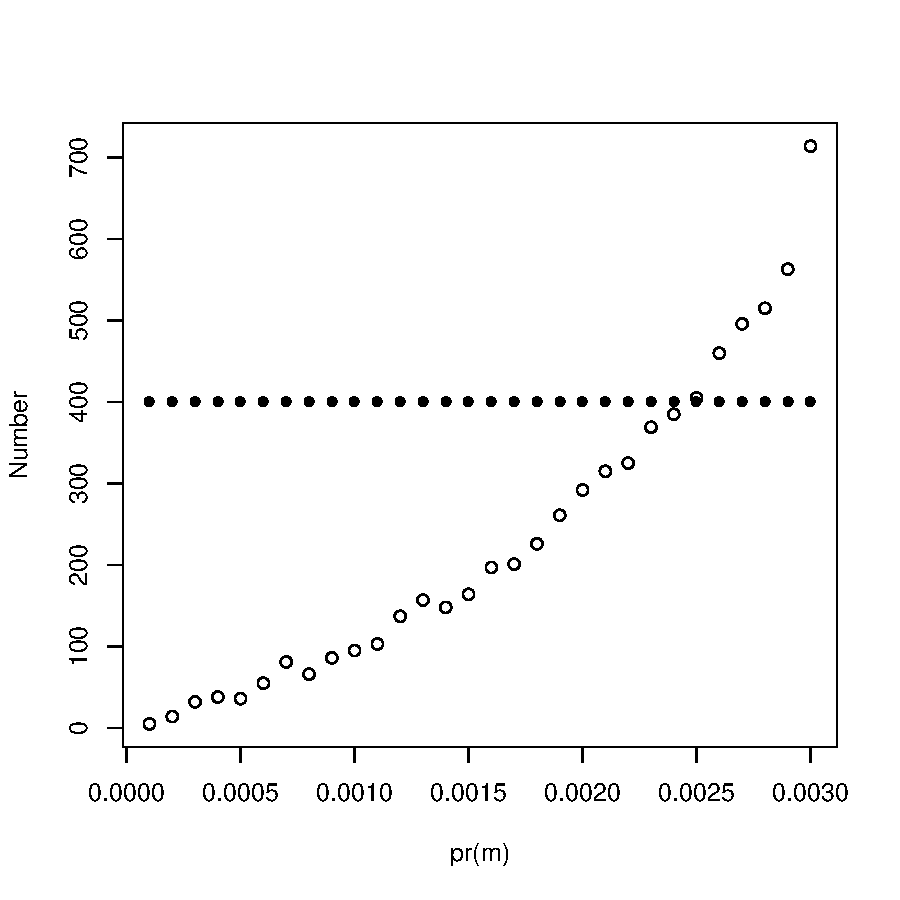
\includegraphics[width=0.375\textwidth]{fig_spob.pdf}
\caption{
The number of species (closed circles; set to $\mathcal S=400$) and objects (open circles) in the interaction matrix as a function of pr($m$).
}
\label{fig_spob}
\end{figure} 

%Interaction types

The ANIMe model consists of four direct interaction types:
$a$: assimilate, which specifies a dependency involving biomass flow,
$n$: need, which specifies a dependency that does not involve biomass flow,
$i$: ignore, the null interaction, and
$m$: make, which connects a species to an object that it engineers. Such objects are interactive components that are made by $\geq 1$ species, and needed, assimilated, or ignored by the others.
We also note that `objects' are to be considered in the abstract, as they could represent actual things a species makes (e.g. an organic molecule), habitat it provides (e.g. as an elephant clears savannas of trees, facilitating shrubs), or even an abiotic condition (e.g. example). 



The four directed interaction types describe specific dependencies that one species/object has on another, however it is the coupling of two opposing directed interactions that describe traditional and familiar ecological relationships (listed in Table 1).
For example, an $a \leftrightarrow i$ interaction describes a typical predator-prey relationship, where species 1 assimilates species 2, and species 2 ignores species 1.
Of course, a prey's abundance does not \emph{ignore} predation, however the ANIMe model operates at the scale of presence-absence, rather than abundance.
Both the $a \leftrightarrow n$ and $n \leftrightarrow n$ interactions describes mutualisms, with the former involving a trophic interaction (such as a plant-pollinator relationship), and the latter without (such as EXAMPLE).
Uniquely, the $m \leftrightarrow n$ interaction describes ecosystem engineering, where a species makes an object, while the presence of the object `needs' the presence of the species that makes it to exist.
As pr($m$) increases, the number of objects made by species increases, such that objects constitute a greater proportion of the interaction matrix compared to the species that create the objects.
Moreover, as pr($m$) increases, the probability that multiple species makes the same object increases, but at a slower rate (FIG).
A complete list of pairwise interactions is found in Table \ref{table_int}.


\begin{table}[h]
  \begin{tabular}{ c  l }
    \hline
    Off-diagonal interactions & Ecological interpretation \\
    \hline
    $a \leftrightarrow i$ & Asymmetric Predation \\
    $a \leftrightarrow a$ & Symmetric predation \\
    $n \leftrightarrow a$ & Trophic mutualism \\
    $n \leftrightarrow n$ & Non-trophic mutualism \\
    $n \leftrightarrow i$ & Commensalism \\
    $i \leftrightarrow i$ & Null \\
    $m \leftrightarrow n$ & Engineering \\
    \hline
  \end{tabular}
  \caption{Pairwise combinations of directed interactions and associated ecological interpretations.}
\end{table}

To establish an interaction matrix, we randomly assign interactions between species and the objects they create based on a set of directed interaction probabilities, which serve as model input. 
Given a species richness $\mathcal S$, the probability that a pair of species have an interaction as listed in Table 1 results from drawing an initial directed interaction ${\rm pr}(a,n,i,m)$, and the conditional probability of drawing the opposing directed interaction, which is constrained due to the fact that not every combination of $[a,n,i,m]$ is feasible.
The emergent $\mathcal R \times \mathcal R$ interaction matrix thus consists of a set of species $\mathcal S$ and objects $\mathcal O$, where $\mathcal R = S + O$. 
Three additional constraints introduce interaction structure to the model:
1) Species and objects behave differently: species can both assimilate and make, whereas objects ignore everything in the system except their `makers'.
2) The distribution of assimilate interactions for a given species (i.e. the trophic degree) is drawn from an exponential distribution, such that the trophic interaction distribution among species is equivalent to that at the heart of the niche model.
3) We introduce a \emph{basal resource} that can be assimilated by species, and those that consume this resource are identified as primary producers.


{\bf Colonization and extinction dynamics}
The interaction matrix above specifies how each species interacts with every other, however not all species are capable of coexisting in a given community at a given time.
Assembly of a species community is thus the result of both colonization and extinction of species that are drawn from the larger interaction matrix, which essentially defines the species pool.

The colonization potential of a given species into a community is determined by two threshold conditions:
1) it must assimilate at least one species/object, which may include the basal resource if that species is a primary producer, and
2) it must satisfy a proportion of its need interactions, given by the threshold $n_t$; higher values of $n_t$ means that entry into the community is more difficult (a higher proportion of need interactions must be satisfied).
If the assimilate and need threshold conditions are both satisfied, colonization is allowed.




The probability of extinction increases sigmoidally as the number of consumers increases for a given species.
Primary extinctions, which are triggered by this \emph{trophic load} can trigger secondary extinctions, as elimination of prey -- and any objects that an eliminated species uniquely makes -- may then result in consumers falling below either of the above threshold conditions.
Accordingly, extinctions cascade until the threshold conditions for every remaining species are satisfied.


\section*{Results \& Discussion}




{\bf Community assembly without extinctions}
In the context of community assembly, the niche space that is created by a given assemblage can be measured by evaluating the number of potential colonizers that can \emph{fit} within the assemblage from the species pool, fulfilling required assimilation and need threshold conditions.
Because colonization without extinction does not account for resource limitation due to ever-expanding trophic loads of species that serve as resources for higher-trophic consumers, niche space is not reduced by packing more species into the community.
However, because colonization from the mainland is a zero-sum event, with each successful colonization the number of potential future colonizers is reduced by one.
Importantly, if a successful colonizer increases the number of potential future colonizers, this can be interpreted as functionally expanding the niche space of the community.




We find that the proportion of the species pool capable of successfully colonizing the assembling community is concave parabolic.
Early in the assembly process, the proportion of potential colonizers is equal to the proportion of species that are primary producers without an abundance of $n$ dependencies (too many need interactions precludes such primary producers from serving as initial colonizers).
As assembly continues, niche space expands to a maximum, and then declines as the species pool diminishes and the community is filled.


%Over pr(m)
For a species pool of $400$, by changing the value of pr($m$) from 0.0001 to 0.002, we alter the proportion of engineers within the pool by multiple orders of magnitude.
As the number of engineers is increased, the number of objects that they create -- and other species can interact with -- is likewise increased.
For example, a single realization where $S=400$ species and pr(m)=$10^{-4}$ resulted in a $412\times412$ interaction matrix (400 species, 12 objects), while a realization with $S=400$ and pr(m)=$0.003$ resulted in a $1200\times1200$ interaction matrix (400 species, 800 objects).
The former example generated a small number of engineers, each producing a single object, whereas the latter example generated a large number of engineers, each producing between 1-6 objects, with a significant minority of objects being produced by multiple engineers.

\begin{figure*}[ht]
\centering
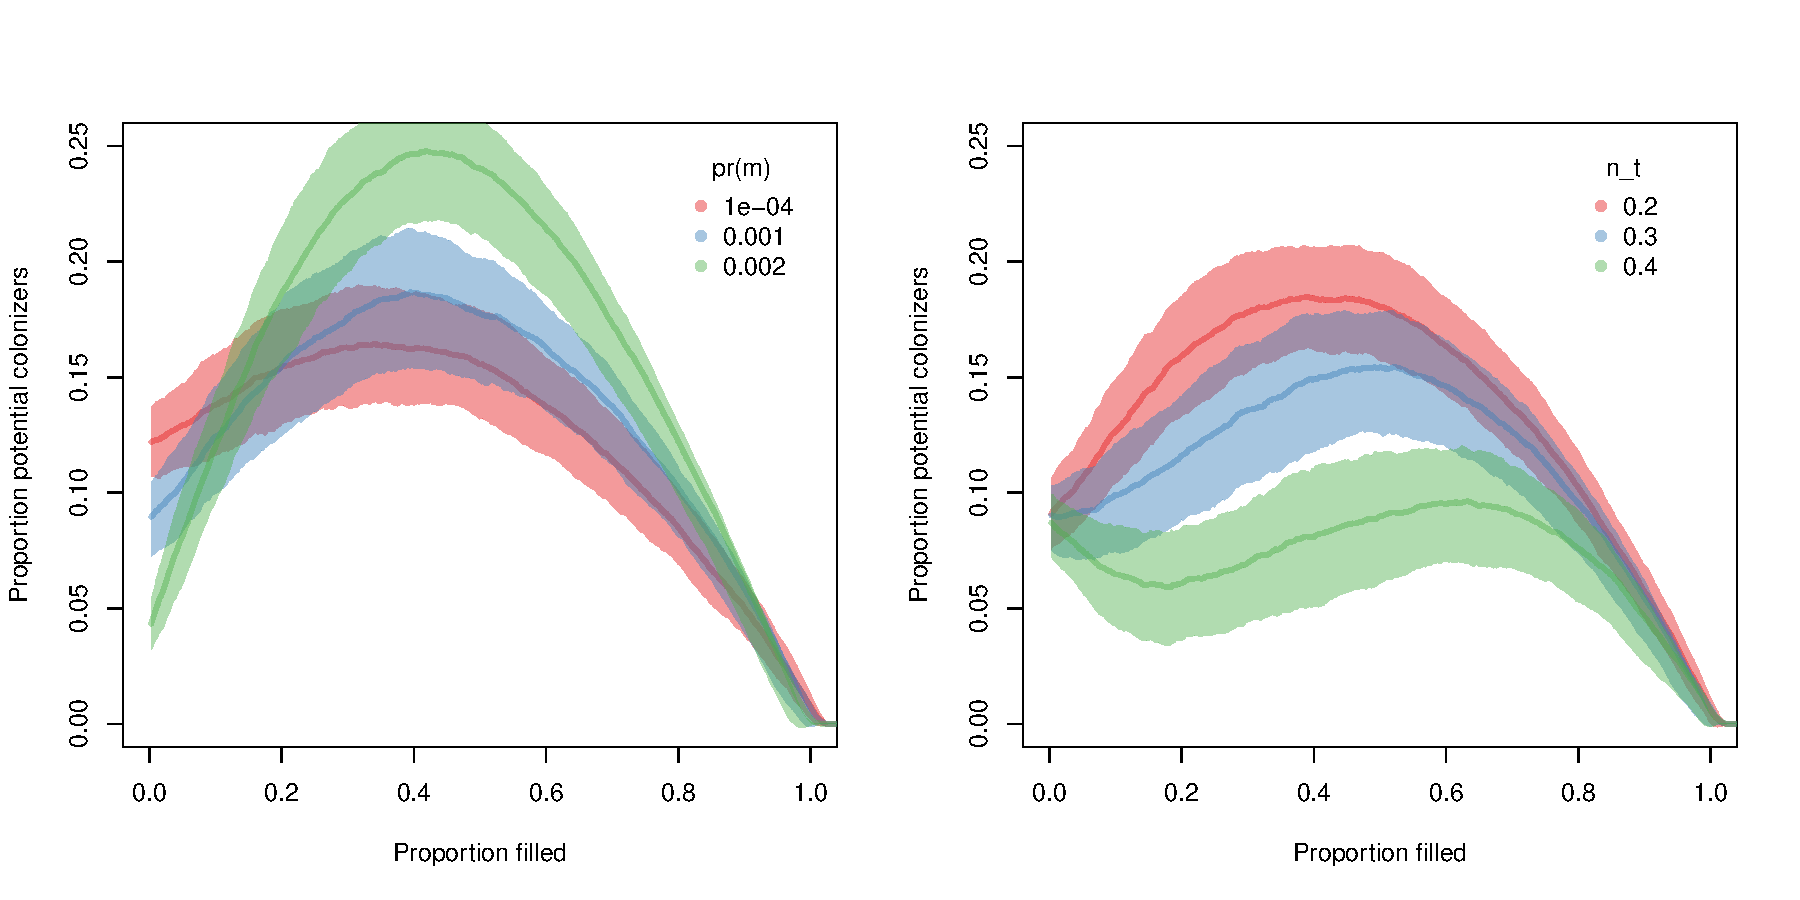
\includegraphics[width=0.75\textwidth]{fig_potcol_comb.pdf}
\caption{
The number of species (closed circles; set to $\mathcal S=400$) and objects (open circles) in the interaction matrix as a function of pr($m$).
}
\label{fig_potcol}
\end{figure*} 

The effects on niche space expansion during assembly, and without the limiting forces of extinction, are substantial.
While both limited-engineering and engineering systems resulted in a concave down niche expansion curve, the engineered system was different in three important ways.
First, the system began assembly with a smaller proportion of potential colonizers.
This is due to the fact that there are many more interdependencies between species and objects, and as there are few objects carried over early in community development, the limitations on species are exaggerated.
Second, the rate that niche space is expanded is higher for engineering communities
Third, the production of objects by engineers increases nearly doubles the potential niche space (proportion of potential future colonizers) midway through assembly.
Once there is a large enough base of colonizers in the assembling communities, there are enough objects present to facilitate rather than inhibit additional colonization opportunities.
Thus, the influence of engineers during assembly - by creating more interdependencies between species and the objects they engineer - both constrains and promotes assembly at different stages of the process.


%Over need_threshold
A species needs at least one assimilate interaction, i.e. it must eat at least one other present species or basal resource, and it must fulfill a certain proportion of its `need' interactions, set by the threshold parameter $n_t$.
As $n_t$ increases, the interdependencies between species become more rigid during the assembly process, and this will serve to limit niche expansion.

However, the trajectory of niche expansion is more complex when $n_t$ is increased.
Rather than simply lowering the proportion of potential colonizers, increasing $n_t$ results in a qualitatively different assembly process where niche space is first lowered, increased, and lowered again as the community is filled.
The initial niche space contraction results from a filling of the initial community with primary producers and their direct consumers.
This lower trophic module fills without creating additional space for higher trophic level organisms due to the harsher restrictions given by a high $n_t$.
Once a critical point in assembly is reached, the potential to add higher trophic level colonizers is attained, and niche space increases to a maximum, only to finally decrease as the species pool is used up.
In some realizations, the community is never able to fill, resulting in a system without higher trophic levels.

Assembly where interdependencies between species (and with moderate engineering) follows a 2-step process.
First, the system is colonized by primary producers.
Second, once the lower trophic levels are filled and reach a critical point, niche expansion permits the additional of higher trophic level colonizers.

%Is there a diversity-stability link here?


%Initial downward slope occurs because primary producers are used up. When it goes back up, there is enough of a base to build a larger community. Will have to check this will average trophic level over time (trophic module!!!)





{\bf Effects of engineers on community richness}
% Negative effects of engineering at the scale of the community
% The effect of engineers on extinction cascade size
Increasing the number of engineers (species with $ `m \leftrightarrow n'$ interactions with their respective objects) at time $t$ results in the potential for marginally larger extinction cascades at time $t+1$.
This weak positive correlation between the number of objects at time $t$ and extinction cascade size at time $t+1$ results from the increasing interconnectedness that results from the higher number of objects relative to species in the system.
Because the existence of a given object is tied to the species that makes them (one or multiple), the effects of primary extinctions are magnified.


% The effect of engineering colonization facilitation
Object richness is strongly positively correlated with the number of potential colonizers.
So from a species packing perspective, engineering enables successful colonization by increasing niche space.


\begin{figure*}[ht]
\centering
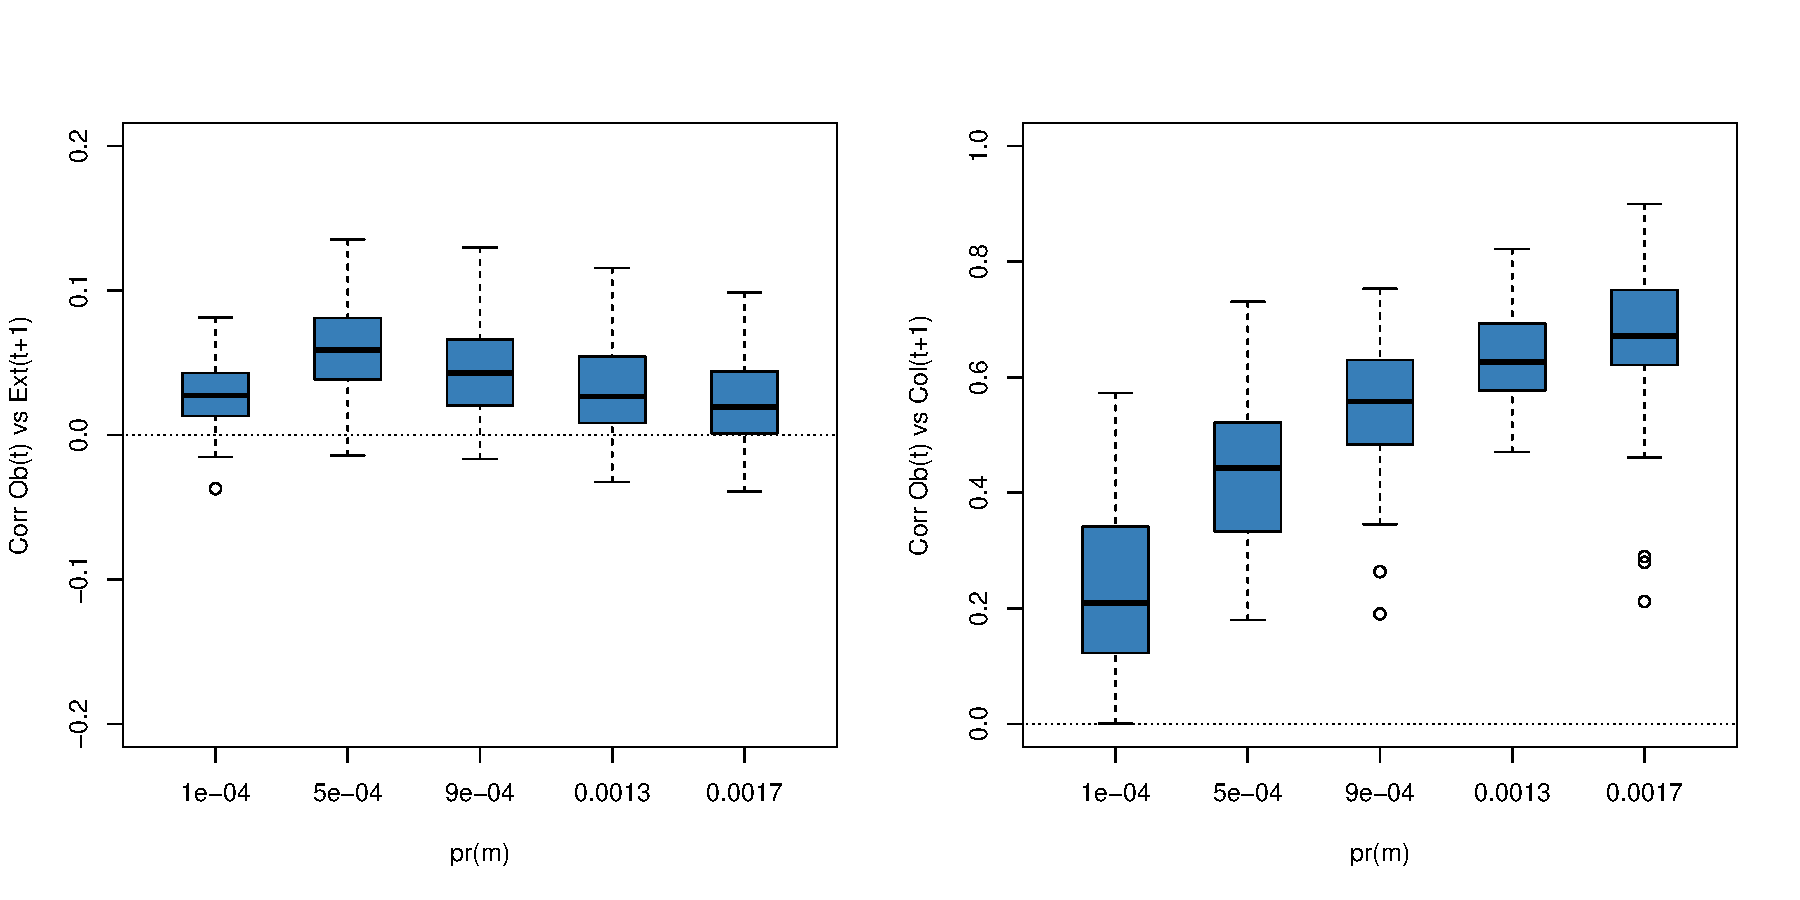
\includegraphics[width=0.75\textwidth]{fig_corrobext_tl2S.pdf}
\caption{
The number of species (closed circles; set to $\mathcal S=400$) and objects (open circles) in the interaction matrix as a function of pr($m$).
}
\label{fig_corrobext}
\end{figure*} 



\end{document}
